\section{Free-Space Management}

%------------------------------------------------
\begin{frame}{The Free-Space Management Problem}

% \begin{columns}[T]

% \column{0.55\textwidth}
\begin{itemize}
    \item Managing free space is simple with fixed-sized units.
    \item Variable-sized allocations make free-space management harder.
    \item The main problem is \textbf{external fragmentation}:
          free memory becomes divided into small, non-contiguous chunks.
    \item An allocation may fail even when the total free space is sufficient.
\end{itemize}

\begin{block}{Key Question}
How should free space be managed to minimize fragmentation while
keeping time and space overheads low?
\end{block}

% \column{0.40\textwidth}
\centering
% Insert figure from page 1 here:
% free / used / free example

% \vspace{1.5cm}
% \fbox{
%     \parbox[c][3.2cm][c]{0.90\linewidth}{
%         \centering
%         Figure: External fragmentation example\\
%         (page 1)
%     }
% }
\begin{figure}
    \centering
    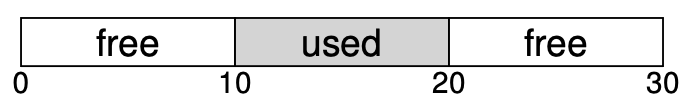
\includegraphics[width=0.8\linewidth]{figs/chapter-17/example-page1.png}
    \caption*{Source: chapter page 1.}
    \label{fig:example-page1-chapter17}
\end{figure}

% \end{columns}

\end{frame}

%------------------------------------------------
\begin{frame}{Assumptions}

\begin{itemize}
    \item Focus on user-level allocators based on \texttt{malloc()} and
          \texttt{free()}.
    \item Free space in the heap is tracked through a \textbf{free list}.
    \item Main concern: \textbf{external fragmentation}.
    \item Allocated memory cannot be relocated; therefore, compaction
          is not available.
    \item Assume a single, contiguous, fixed-size heap.
\end{itemize}

\end{frame}

%------------------------------------------------
\begin{frame}{Splitting}

% \begin{columns}[T]

% \column{0.52\textwidth}
\begin{itemize}
    \item A free list records the available chunks of memory.
    \item If a request is smaller than an available free chunk,
          the allocator can \textbf{split} that chunk.
    \item One part is returned to the caller.
    \item The remaining part stays on the free list.
\end{itemize}

% \column{0.43\textwidth}
\centering

% \fbox{
%     \parbox[c][3.8cm][c]{0.90\linewidth}{
%         \centering
%         Figure: Free list before and after splitting\\
%         (pages 3--4)
%     }
% }

% \vspace{0.2cm}

\begin{figure}
    \centering
    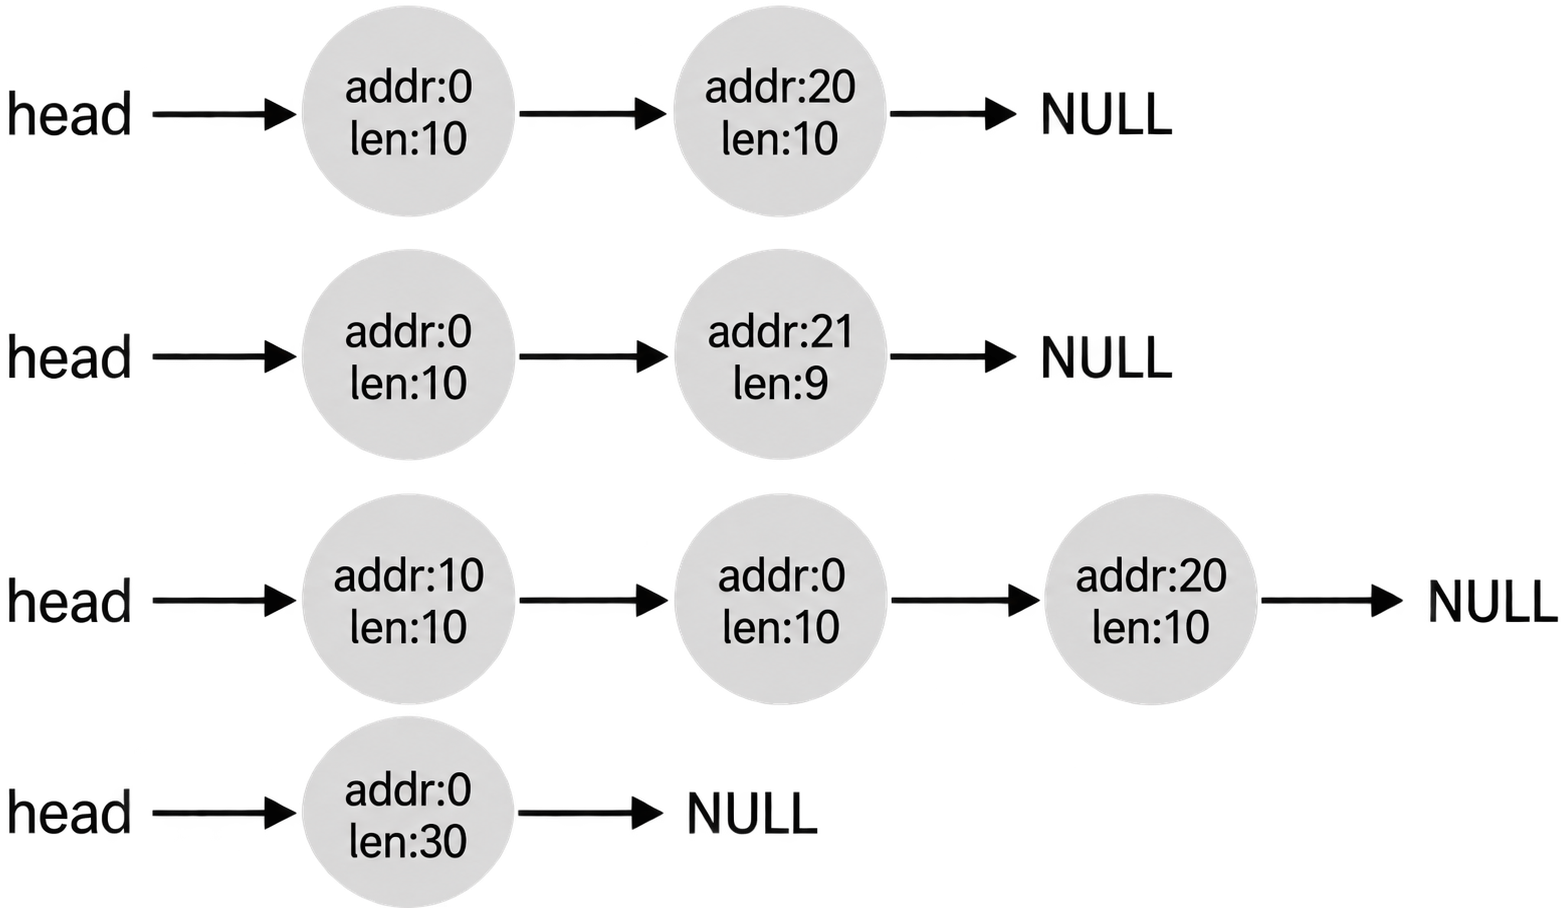
\includegraphics[width=0.8\linewidth]{figs/chapter-17/free-list.png}
    % \caption{Caption}
    \label{fig:free-list}
\end{figure}

\end{frame}

%------------------------------------------------
\begin{frame}{Coalescing}

% \begin{columns}[T]

% \column{0.52\textwidth}
\begin{itemize}
    \item When memory is freed, simply inserting it into the free list
          can leave adjacent free chunks separated.
    \item \textbf{Coalescing} merges neighboring free chunks.
    \item This helps preserve larger contiguous regions of free memory.
\end{itemize}

% \column{0.43\textwidth}
% \centering

% \fbox{
%     \parbox[c][3.8cm][c]{0.90\linewidth}{
%         \centering
%         Figure: Free list before and after coalescing\\
%         (page 4)
%     }
% }

% \end{columns}

\end{frame}

%------------------------------------------------
\begin{frame}{Tracking Allocated Regions}

\begin{columns}[T]

\column{0.52\textwidth}
\begin{itemize}
    \item \texttt{free(ptr)} receives a pointer, but not the allocation size.
    \item Allocators store metadata in a \textbf{header} immediately before
          the allocated region.
    \item The header can contain:
    \begin{itemize}
        \item allocation size;
        \item a magic number;
        \item additional metadata.
    \end{itemize}
    \item Pointer arithmetic allows \texttt{free()} to locate the header.
\end{itemize}

\column{0.43\textwidth}
\centering

% \fbox{
%     \parbox[c][4.2cm][c]{0.90\linewidth}{
%         \centering
%         Figures 17.1 and 17.2\\
%         Allocated region and header\\
%         (page 5)
%     }
% }
\begin{figure}
    \centering
    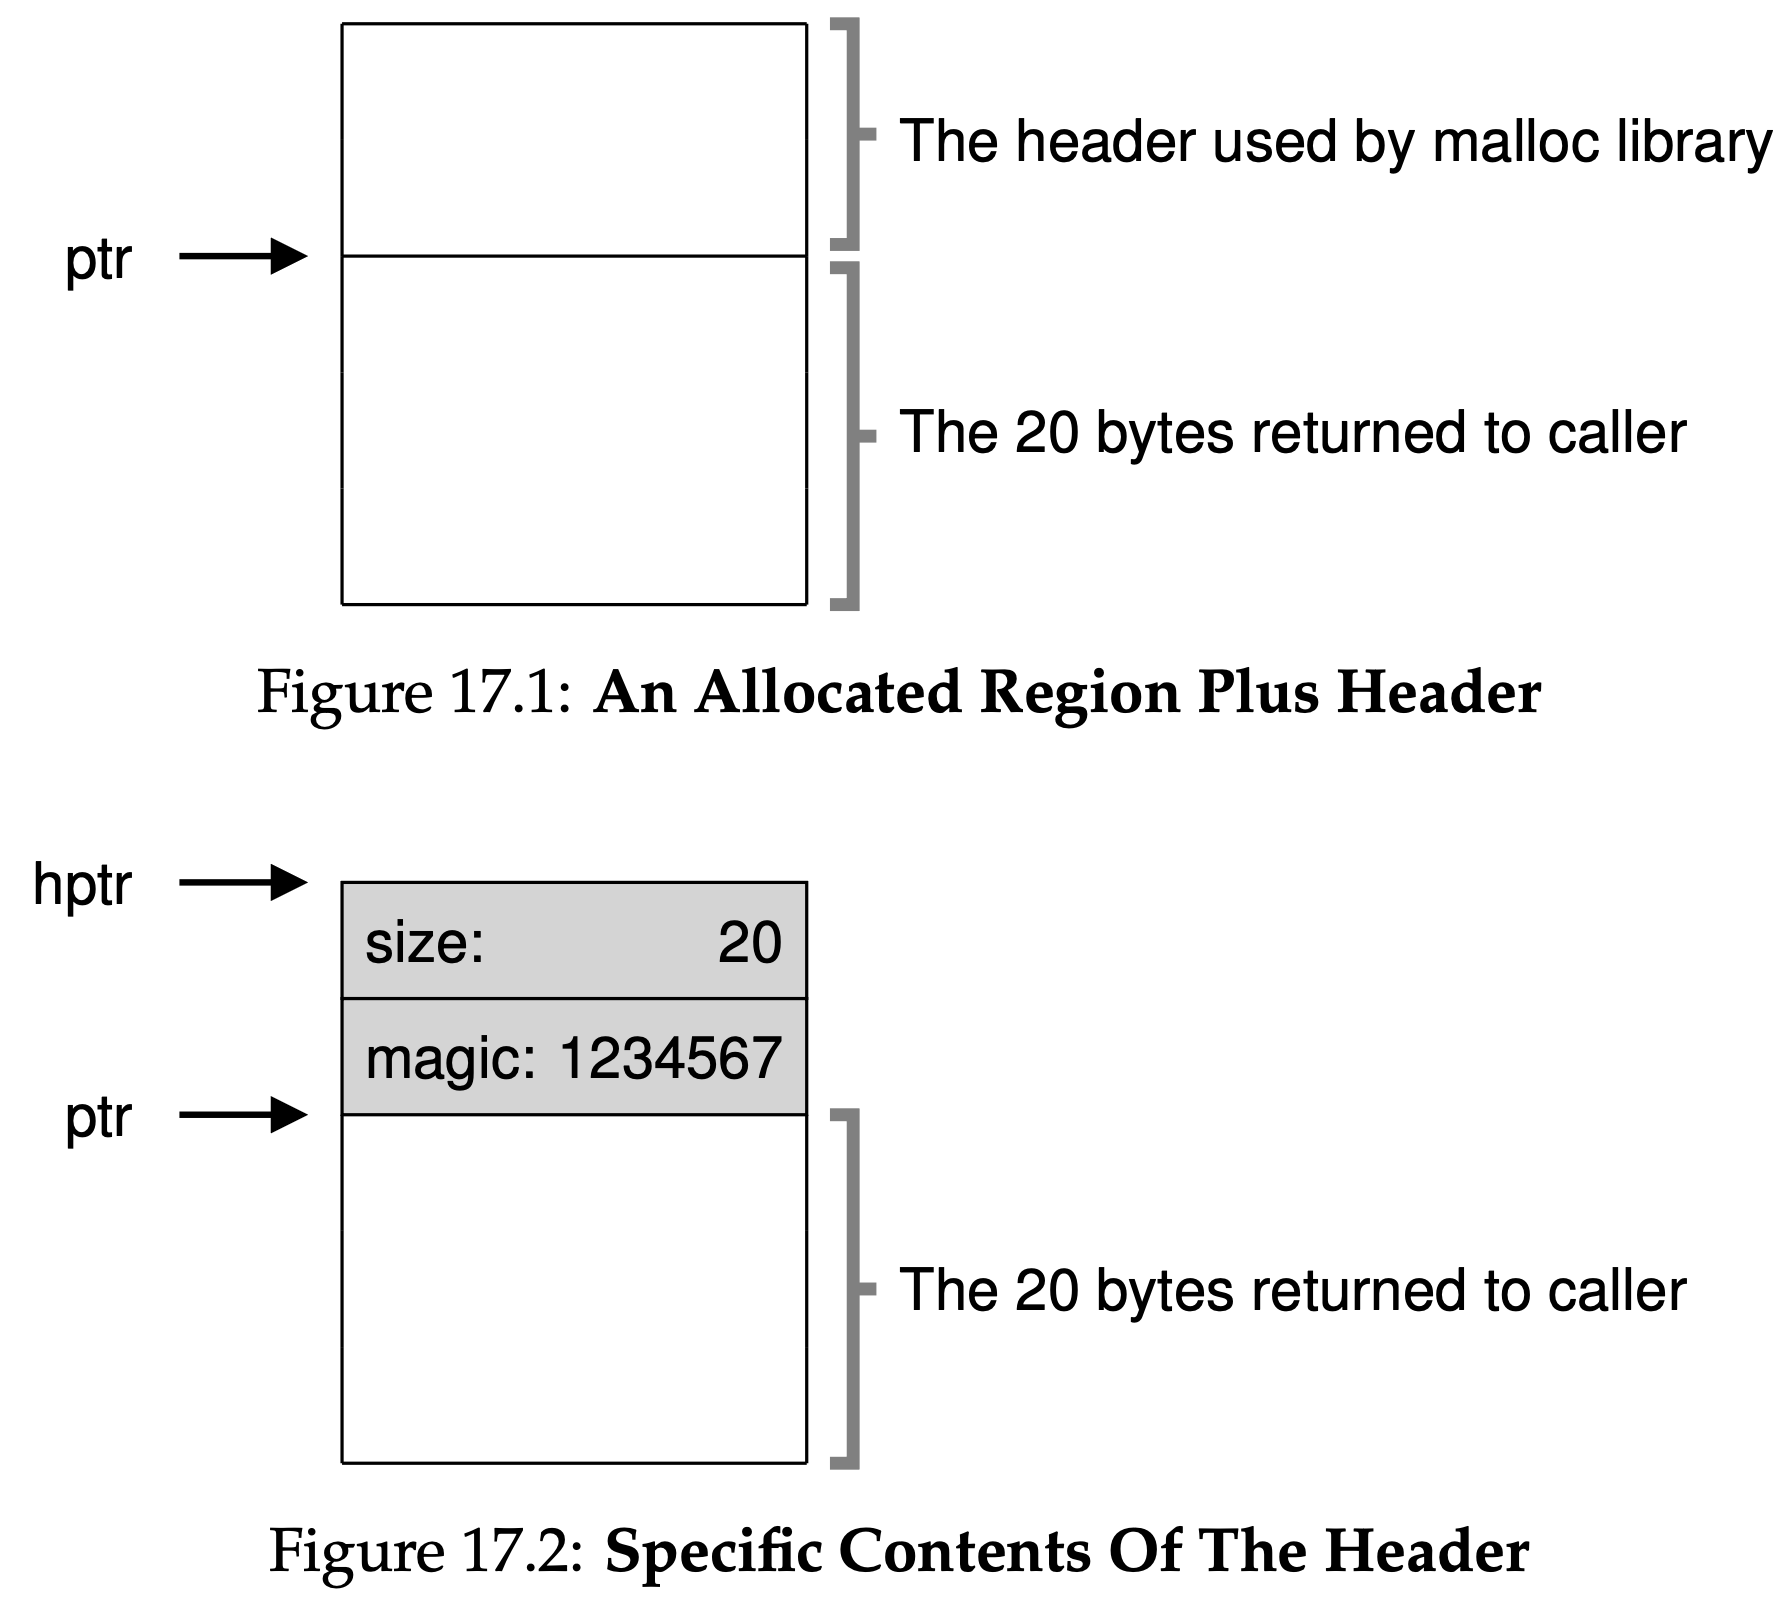
\includegraphics[width=1.1\linewidth]{figs/chapter-17/figures-17.1-17.2.png}
    \caption*{Source: chapter page 5.}
    \label{fig:figures-17.1-17.2}
\end{figure}

\end{columns}

\end{frame}

%------------------------------------------------
\begin{frame}{Locating the Header}

% \begin{columns}[T]idth}

\begin{block}{Pointer Arithmetic}
\texttt{header\_t *hptr = (header\_t *) ptr - 1;}
\end{block}

\begin{itemize}
    \item The header is stored immediately before the pointer returned
          to the application.
    \item The allocator can recover the allocation size from the header.
    \item Thus, a request for $N$ bytes requires space for:
\end{itemize}

\[
N + \text{sizeof(header)}
\]

% \column{0.40\textwidth}
% \centering

% \fbox{
%     \parbox[c][3.8cm][c]{0.90\linewidth}{
%         \centering
%         Figure 17.2\\
%         Header and user-visible pointer\\
%         (page 5)
%     }
% }

% \end{columns}

\end{frame}

%------------------------------------------------
\begin{frame}{Embedding the Free List}

\begin{columns}[T]

\column{0.52\textwidth}
\begin{itemize}
    \item The allocator cannot call \texttt{malloc()} to create
          free-list nodes.
    \item Free-list metadata must therefore be stored
          \textbf{inside the free memory itself}.
    \item Initially, the heap can be represented by a single free node.
    \item The chapter illustrates this using a 4096-byte heap.
\end{itemize}

\column{0.43\textwidth}
\centering

% \fbox{
%     \parbox[c][4.0cm][c]{0.90\linewidth}{
%         \centering
%         Figure 17.3\\
%         Heap with one free chunk\\
%         (page 7)
%     }
% }
\begin{figure}
    \centering
    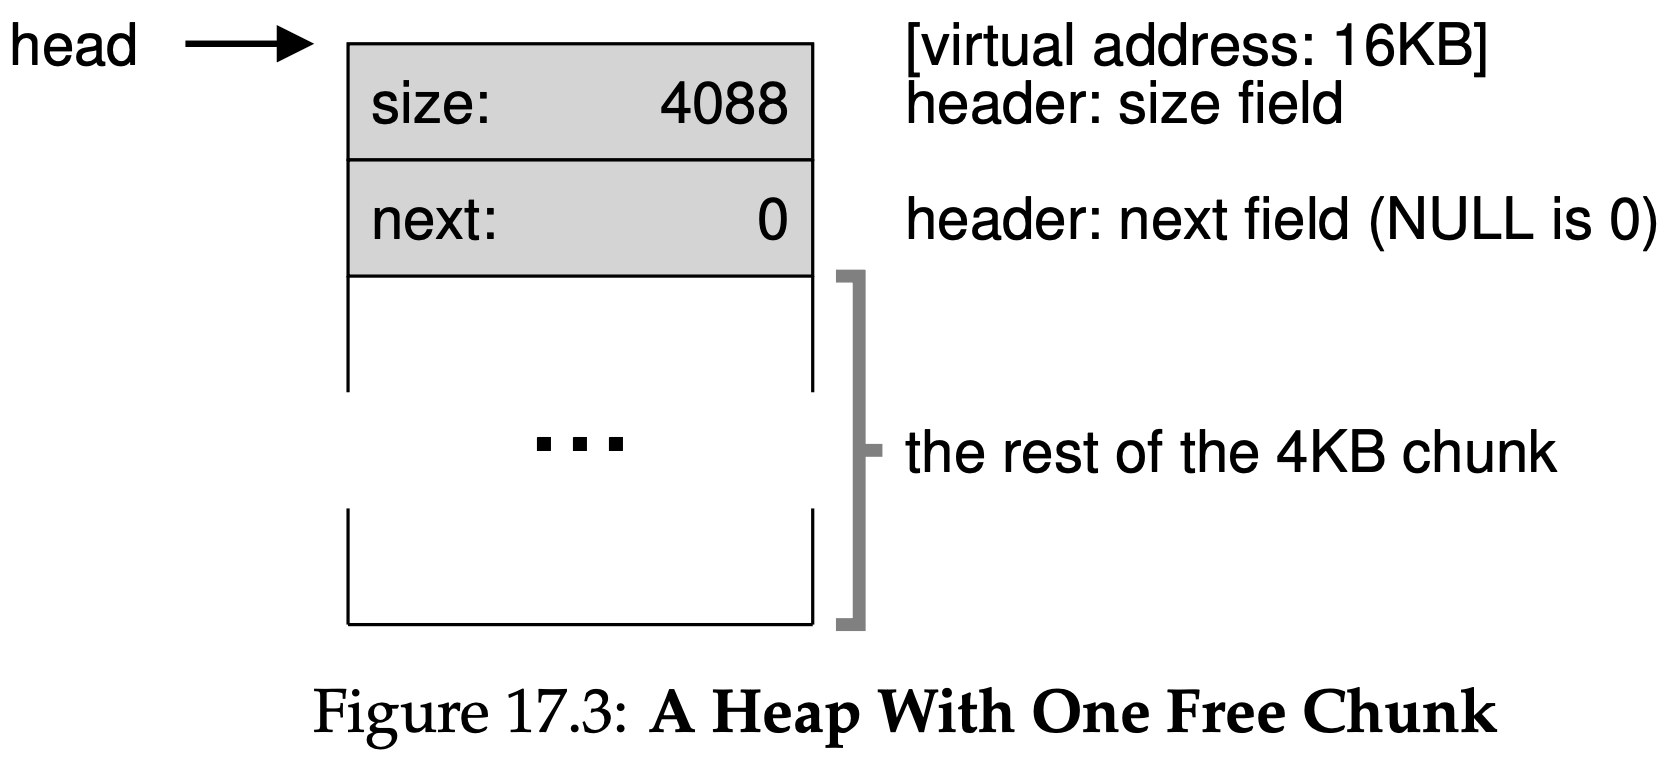
\includegraphics[width=1.1\linewidth]{figs/chapter-17/figure-17.3.png}
    \caption*{Source: chapter page 7.}
    \label{fig:figure-17.3}
\end{figure}

\end{columns}

\end{frame}

%------------------------------------------------
\begin{frame}{After One Allocation}

\begin{columns}[T]

\column{0.50\textwidth}
\begin{itemize}
    \item Suppose the application requests 100 bytes.
    \item The allocator selects the available free chunk.
    \item The chunk is split into:
    \begin{itemize}
        \item an allocated region plus its header;
        \item the remaining free region.
    \end{itemize}
    \item With an 8-byte header, 108 bytes are consumed.
\end{itemize}

\column{0.45\textwidth}
\centering

% \fbox{
%     \parbox[c][4.0cm][c]{0.90\linewidth}{
%         \centering
%         Figure 17.4\\
%         Heap after one allocation\\
%         (page 7)
%     }
% }

\begin{figure}
    \centering
    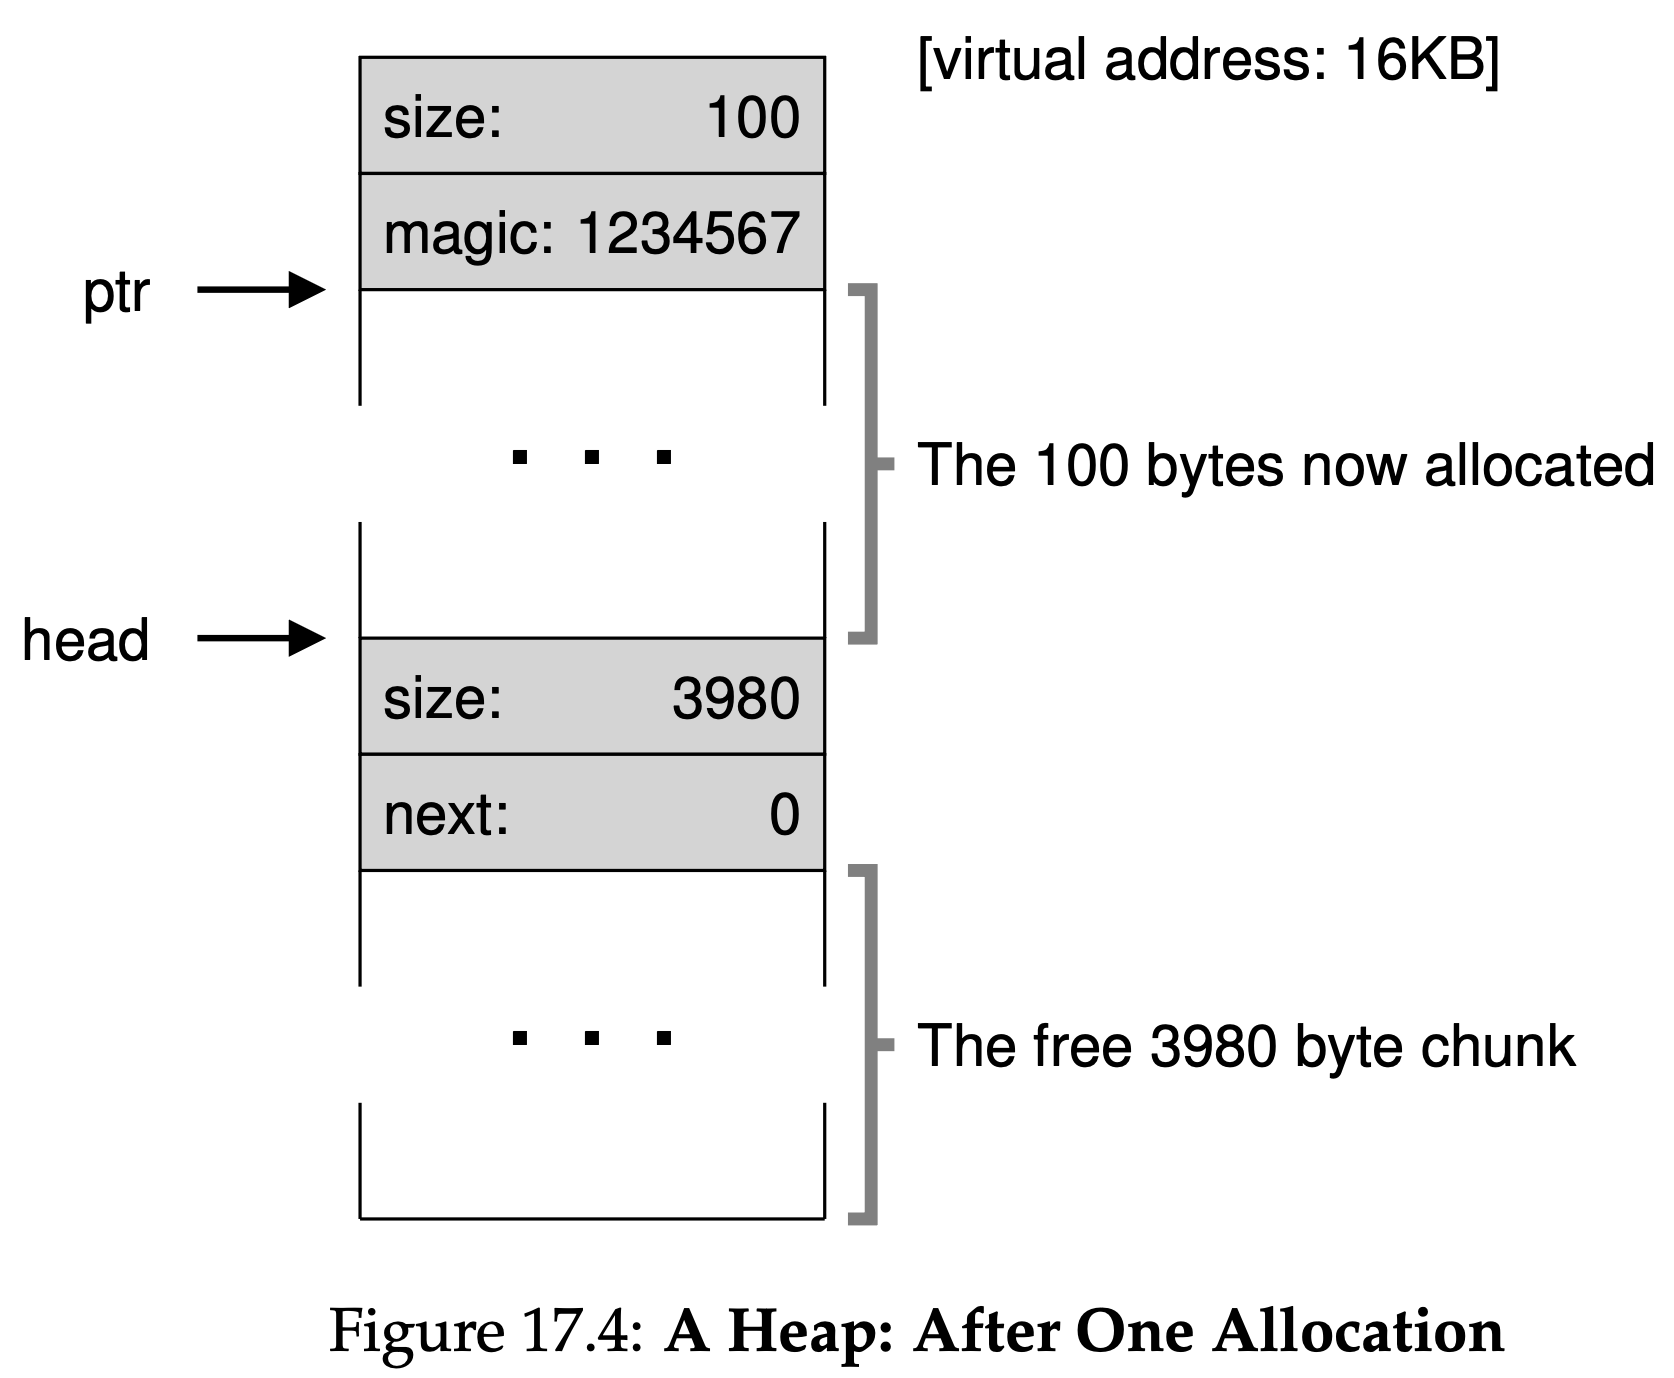
\includegraphics[width=1.1\linewidth]{figs/chapter-17/figure-17.4.png}
    \caption*{Source: chapter page 7.}
    \label{fig:figure-17.4}
\end{figure}

\end{columns}

\end{frame}

%------------------------------------------------
\begin{frame}{Free-List Evolution}

% \begin{columns}[T]

% \column{0.48\textwidth}
\begin{itemize}
    \item Repeated allocations progressively split the free region.
    \item When one block is freed, it is inserted back into the free list.
    \item The free list may therefore contain several non-contiguous chunks.
\end{itemize}

% \column{0.48\textwidth}
% \centering

% \fbox{
%     \parbox[c][4.2cm][c]{0.90\linewidth}{
%         \centering
%         Figures 17.5 and 17.6\\
%         Three allocated chunks and\\
%         freeing the middle chunk\\
%         (pages 8--9)
%     }
% }

% \end{columns}

\begin{columns}
    \begin{column}{0.48\textwidth}
        \begin{figure}
        \centering
        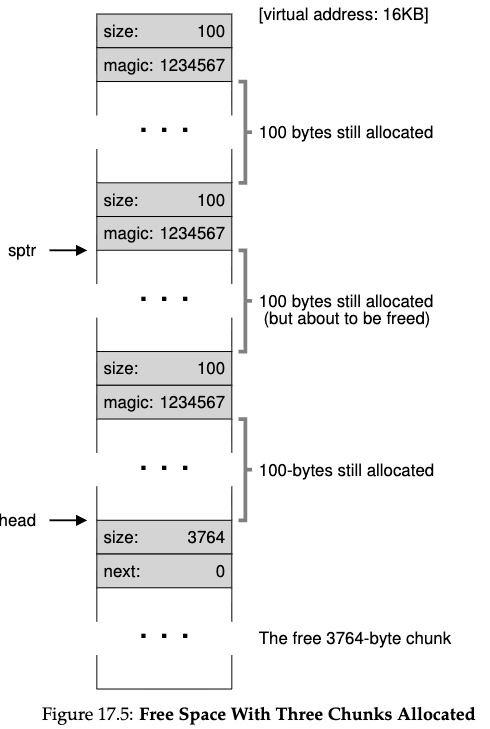
\includegraphics[width=0.7\linewidth]{figs/chapter-17/figure-17.5.png}
        \caption*{Source: chapter page 8.}
        \label{fig:figure-17.5}
        \end{figure}        
    \end{column}
    \begin{column}{0.48\textwidth}
        \begin{figure}
        \centering
        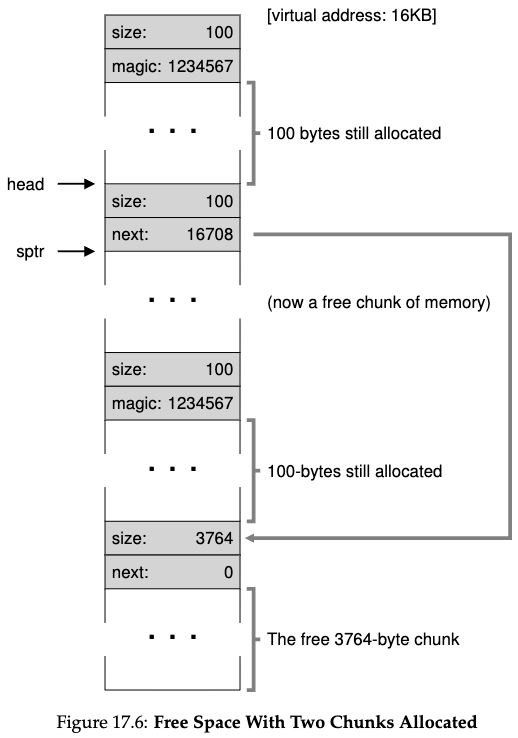
\includegraphics[width=0.7\linewidth]{figs/chapter-17/figure-17.6.png}
        \caption*{Source: chapter page 9.}
        \label{fig:figure-17.6}
        \end{figure}
    \end{column}
\end{columns}

\end{frame}

%------------------------------------------------
\begin{frame}{Why Coalescing Matters}

\begin{columns}[T]

\column{0.50\textwidth}
\begin{itemize}
    \item If all allocated regions are freed without coalescing,
          the free list can remain fragmented.
    \item The heap may be entirely free but still represented as
          multiple separate chunks.
    \item Adjacent chunks must therefore be merged.
\end{itemize}

\column{0.45\textwidth}
\centering

\begin{figure}
    \centering
    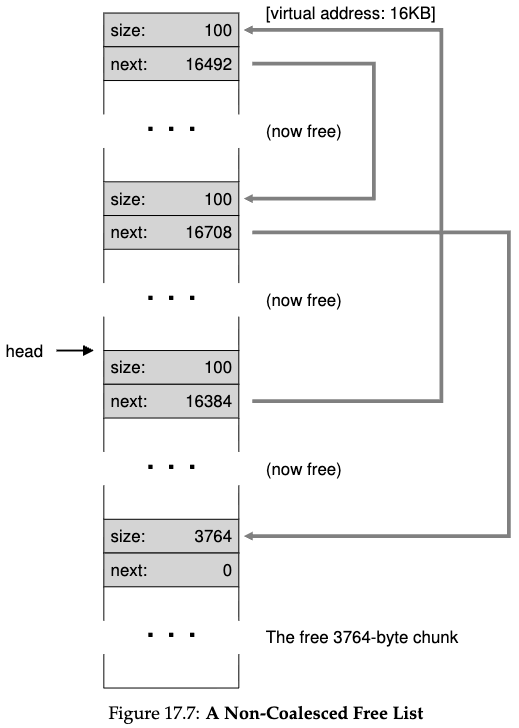
\includegraphics[width=1.0\linewidth]{figs/chapter-17/figure-17.7.png}
    \caption*{Source: chapter page 10.}
    \label{fig:figure-17.7}
\end{figure}

% \fbox{
%     \parbox[c][4.0cm][c]{0.90\linewidth}{
%         \centering
%         Figure 17.7\\
%         Non-coalesced free list\\
%         (page 10)
%     }
% }

\end{columns}

\end{frame}

%------------------------------------------------
\begin{frame}{Growing the Heap}

\begin{itemize}
    \item If no suitable free space remains, the allocator may return
          \texttt{NULL}.
    \item Traditional allocators can instead request more memory from
          the operating system.
    \item UNIX systems historically use mechanisms such as \texttt{sbrk()}.
    \item The OS maps additional physical pages into the process address space,
          increasing the heap size.
\end{itemize}

\end{frame}

%------------------------------------------------
\begin{frame}{Basic Allocation Strategies}

\begin{columns}[T]

\column{0.55\textwidth}

\begin{description}
    \item[Best Fit] Smallest free chunk that satisfies the request.
    \item[Worst Fit] Largest available free chunk.
    \item[First Fit] First chunk large enough for the request.
    \item[Next Fit] Continue the first-fit search from the previous position.
\end{description}

\medskip

\begin{itemize}
    \item Strategies trade off search cost and fragmentation.
\end{itemize}

\column{0.40\textwidth}
\centering

% \fbox{
%     \parbox[c][3.8cm][c]{0.90\linewidth}{
%         \centering
%         Free-list example\\
%         $10 \rightarrow 30 \rightarrow 20$\\
%         Request: 15 bytes\\
%         (pages 12--13)
%     }
% }

\vspace{1cm}

\begin{figure}
    \centering
    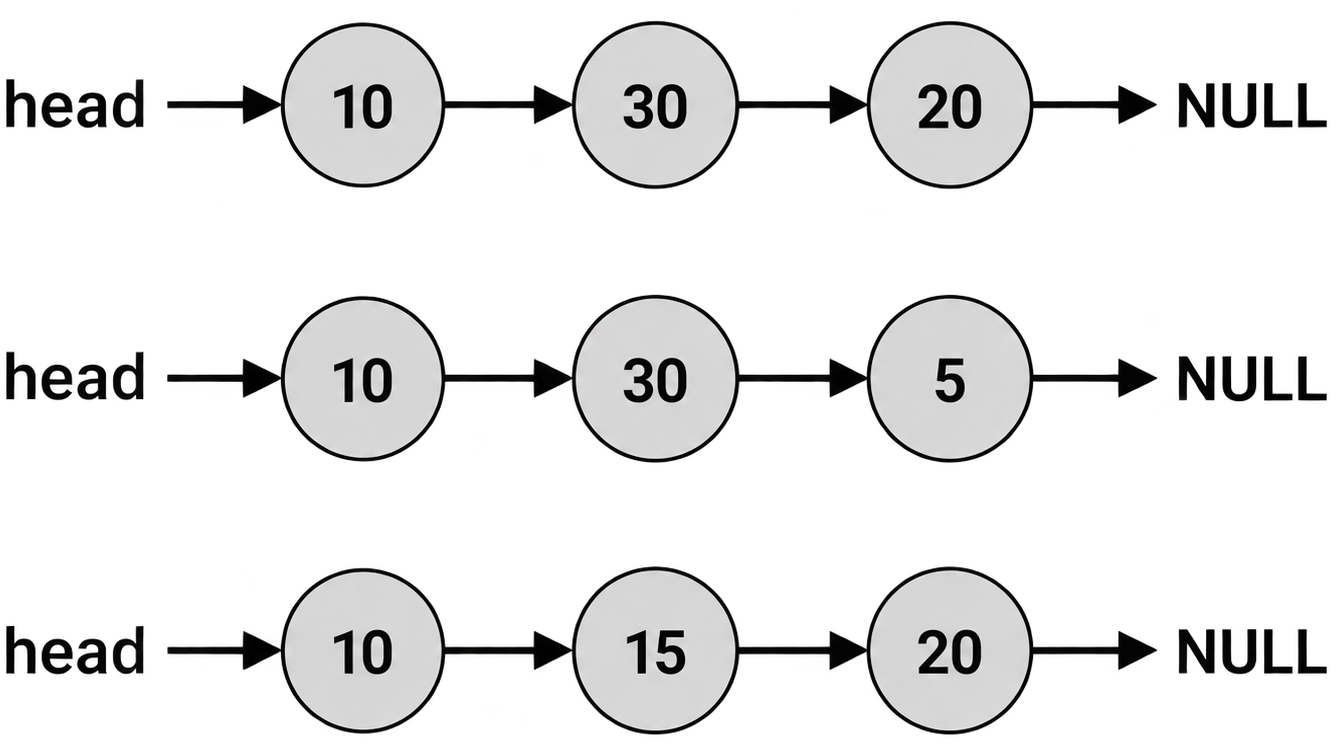
\includegraphics[width=1.0\linewidth]{figs/chapter-17/best-worst-first-next-fit.png}
    % \caption{Caption}
    \label{fig:placeholder}
\end{figure}

\end{columns}

\end{frame}

%------------------------------------------------
\begin{frame}{Segregated Lists}

% \begin{columns}[T]

% \column{0.55\textwidth}
\begin{itemize}
    \item Maintain separate free lists for frequently requested object sizes.
    \item Requests of those sizes can be served quickly.
    \item Fragmentation becomes less of a concern within the specialized pool.
    \item The \textbf{slab allocator} applies this idea to frequently used
          kernel objects.
    \item Freed objects can remain initialized, reducing initialization
          and destruction overhead.
\end{itemize}

% \column{0.40\textwidth}
% \centering

% \fbox{
%     \parbox[c][3.8cm][c]{0.90\linewidth}{
%         \centering
%         Optional diagram:\\
%         specialized object caches / slabs\\
%         based on the description\\
%         from pages 13--14
%     }
% }

% \end{columns}

\end{frame}

%------------------------------------------------
\begin{frame}{Buddy Allocation}

\begin{columns}[T]

\column{0.50\textwidth}
\begin{itemize}
    \item Memory begins as one block of size $2^N$.
    \item Blocks are recursively divided in half until a suitable block
          is found.
    \item Allocations therefore use power-of-two-sized blocks.
    \item When a block is freed, its \textbf{buddy} can be identified
          and merged efficiently.
    \item This simplifies coalescing, but may introduce
          \textbf{internal fragmentation}.
\end{itemize}

\column{0.45\textwidth}
\centering

\begin{figure}
    \centering
    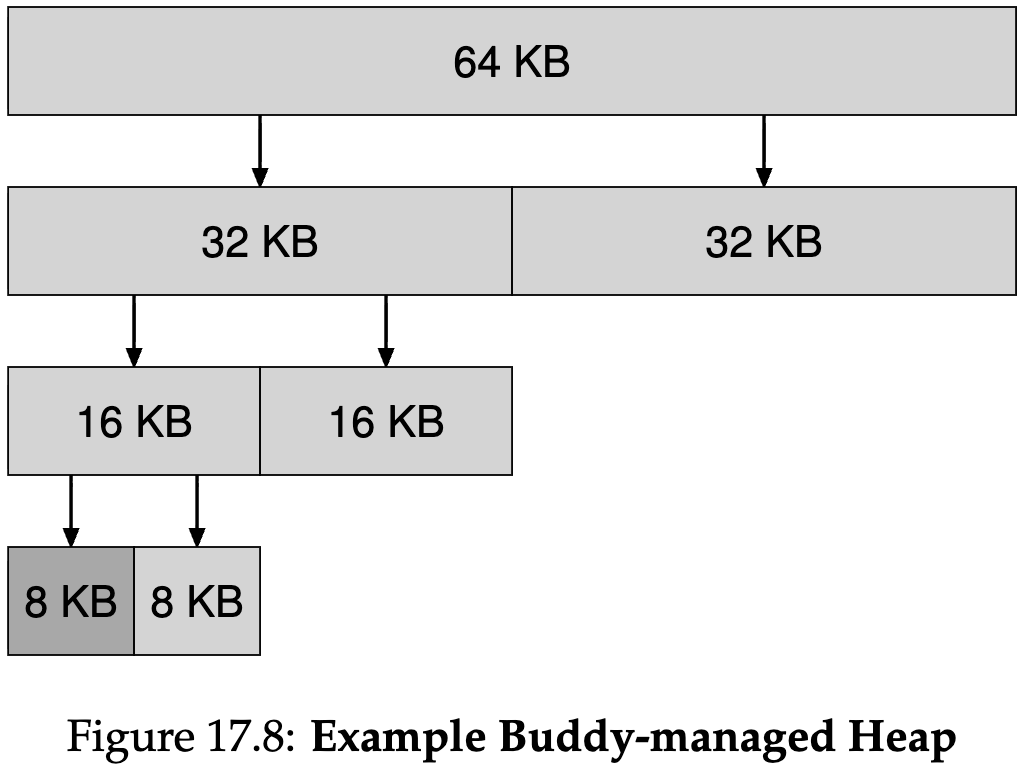
\includegraphics[width=1.1\linewidth]{figs/chapter-17/figure-17.8.png}
    \caption*{Source: chapter page 15.}
    \label{fig:figure-17.8}
\end{figure}

% \fbox{
%     \parbox[c][4.4cm][c]{0.90\linewidth}{
%         \centering
%         Figure 17.8\\
%         Buddy-managed heap\\
%         $64\,KB \rightarrow 32\,KB \rightarrow 16\,KB
%         \rightarrow 8\,KB$\\
%         (page 15)
%     }
% }

\end{columns}

\end{frame}

%------------------------------------------------
\begin{frame}{Other Ideas}

\begin{itemize}
    \item Simple free-list searches do not always scale well.
    \item More advanced allocators may use:
    \begin{itemize}
        \item balanced binary trees;
        \item splay trees;
        \item partially ordered trees.
    \end{itemize}
    \item Modern allocators must also perform well on multiprocessor
          and multithreaded systems.
\end{itemize}

\end{frame}

%------------------------------------------------
\begin{frame}{Summary}

\begin{itemize}
    \item Variable-sized allocation introduces \textbf{external fragmentation}.
    \item \textbf{Splitting} and \textbf{coalescing} are fundamental mechanisms.
    \item Headers allow the allocator to recover allocation metadata.
    \item Free-list organization directly affects allocation behavior.
    \item Best fit, worst fit, first fit, and next fit provide different
          allocation policies.
    \item Segregated lists and buddy allocation offer alternative approaches.
    \item Fast, space-efficient, and scalable allocation remains a challenging
          systems problem.
\end{itemize}

\end{frame}